\documentclass{beamer}
\hypersetup{pdfpagemode=FullScreen}
\usetheme{CambridgeUS}
\usecolortheme{dolphin}
\usefonttheme{serif}
\usepackage{microtype}
\usepackage[utf8]{inputenc}
\usepackage{graphicx}
\usepackage{mathtools}
\usepackage{breqn}
\usepackage{empheq}
\usepackage{tensor}
\usepackage{array}
\usepackage{multirow}
\usepackage{transparent}
\usepackage{fontenc}
\usepackage{booktabs}
\usepackage{natbib}
\usepackage{hyperref}
\usepackage{listings}
\usepackage{tikz}
\usepackage{graphicx}
\usepackage{subcaption}
\usetikzlibrary{shapes.geometric, arrows}
\usepackage{enumerate}
\setbeamertemplate{navigation symbols}{}
% set colors
\definecolor{myNewColorA}{RGB}{51,132,203}
\definecolor{myNewColorB}{RGB}{229,165,70}
\definecolor{myNewColorC}{RGB}{226,182,0}
\setbeamercolor*{palette primary}{bg=myNewColorA, fg=white}
\setbeamercolor*{palette secondary}{bg=myNewColorB, fg=black}
\setbeamercolor*{palette tertiary}{bg=myNewColorB, fg=black}
\setbeamercolor*{titlelike}{fg=myNewColorA}
\setbeamercolor*{title}{bg=myNewColorA, fg=white}
\setbeamercolor*{item}{fg=myNewColorA}
\setbeamercolor*{caption name}{fg=myNewColorA}

\lstset{
  language=C,
  basicstyle=\ttfamily\footnotesize,
  keywordstyle=\bfseries\color{blue},
  commentstyle=\itshape\color{green!60!black},
  stringstyle=\color{red},
  numbers=left,
  numberstyle=\tiny\color{gray},
  stepnumber=1,
  numbersep=5pt,
  frame=single,
  rulecolor=\color{black},
  tabsize=4,
  breaklines=true,
  showstringspaces=false,
  captionpos=b
}

% define envoirenmemt
\newenvironment{tres important}[2][]{
	\setkeys{EmphEqEnv}{#2}
	\setkeys{EmphEqOpt}{box={\setlength{\fboxsep}{10pt}\fcolorbox{myNewColorA}{white}},#1}
	\EmphEqMainEnv}
{\endEmphEqMainEnv}
%------------------------------------------------------------

% To use the other logo of University use following: .......
%\titlegraphic{\includegraphics[height=3cm]{figures/UWA_V_logo.png}}

\setbeamerfont{title}{size=\large}
\setbeamerfont{subtitle}{size=\small}
\setbeamerfont{author}{size=\large}
\setbeamerfont{date}{size=\small}
\setbeamerfont{institute}{size=\large}


\author[Chayan Pathak,M.Tech,CSE]{Chayan Pathak\\12310630\\M.Tech CSE \\ \textbf{Supervisor:} Dr. Dhiman Saha}
\title[Thesis Defence Seminar]{Injecting Chaos: Fault Attack Setup and Analysis Via ChipWhisperer}
\date[10/06/2025]

%------------------------------------------------------------
%This block of commands puts the table of contents at the 
%beginning of each section and highlights the current section:
\AtBeginSection[]
{
  \begin{frame}
    \frametitle{Contents}
    \tableofcontents[currentsection]
  \end{frame}
}
\AtBeginSection[]{
  \begin{frame}
  \vfill
  \centering
  \begin{beamercolorbox}[sep=8pt,center,shadow=true,rounded=true]{title}
    \usebeamerfont{title}\insertsectionhead\par%
  \end{beamercolorbox}
  \vfill
  \end{frame}
}
%------------------------------------------------------------
\begin{document}
%The next statement creates the title page.
%\frame{\titlepage}

\begin{frame}
        \begin{figure}
	\centering
	
\includegraphics[width=0.2\linewidth]{images/iitbhilailogo.png}
	\label{fig:iitlogo}
        \end{figure}
    
            \titlepage
            
        \end{frame}
        \begin{frame}{Research Timeline}
          \begin{center}
              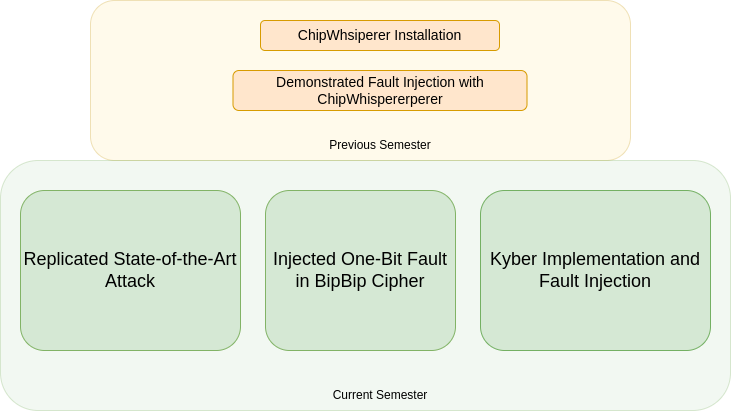
\includegraphics[width=1\linewidth]{images/mtech.drawio.png}
              
          \end{center}
        \end{frame}
        \begin{frame}
            \frametitle{Contents}
            \tableofcontents
        \end{frame}

%------------------------------------------------------------

\section{Introduction To Fault Attacks}
\begin{frame}
 % \frametitle{What is a Fault Injection Attack?}

  \begin{itemize}
    \item \textbf{Fault Injection Attacks (FIA)} are hardware-based attacks that introduce faults into a system to alter its behavior.
    \item Attackers induce transient errors to bypass security checks, alter data or extract sensitive data.
    \item Common techniques:
    \begin{itemize}
        \item Voltage Glitching
        \item Clock Glitching
        \item Electromagnetic (EM) Pulses
        \item Laser Fault Injection
    \end{itemize}
    \item Often used to target cryptographic algorithms (e.g., AES, RSA).
  \end{itemize}
\end{frame}


\section{Setting Up a Fault Injection Lab with ChipWhisperer}

\begin{frame}
  %\frametitle{Setting Up a Fault Injection Lab with ChipWhisperer}

  \begin{itemize}
    \item \textbf{ChipWhisperer} is an open-source toolchain for side-channel and fault injection research.
    \item Designed for teaching reasearch and evaluating hardware security.
    \item Includes:
    \begin{itemize}
        \item CWNano,CWLite or CWHusky hardware for capturing traces.
        \item Target board (e.g., XMEGA, STM32, SAM4S).
        \item Software suite for glitching, capturing, and analysis.
    \end{itemize}
    \item Supports fault injection via:
    \begin{itemize}
        \item Clock Glitching
        \item Voltage Faults
        \item Electromagnetic Pulse Injection (with add-ons like ChipShouter)
    \end{itemize}
  \end{itemize}
\end{frame}

\begin{frame}{Hardware Setup}
  \centering
  \begin{minipage}[b]{0.3\linewidth}
    \centering
    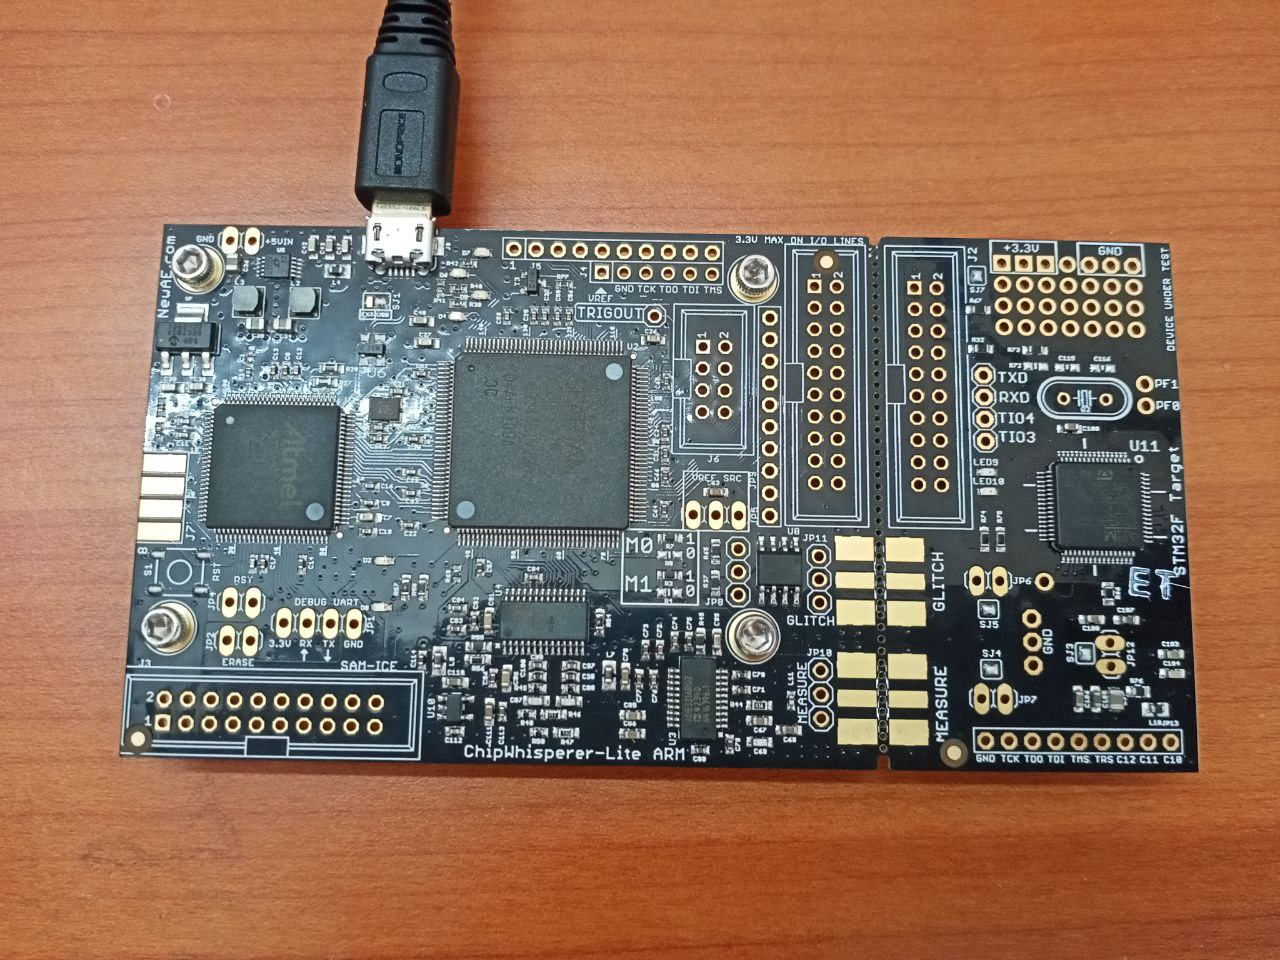
\includegraphics[width=\linewidth]{images/cwlite_background.JPEG}
    \smallskip
    \textbf{CWNLite with ARM 32-bit Target}
  \end{minipage}
  \hfill
  \begin{minipage}[b]{0.3\linewidth}
    \centering
    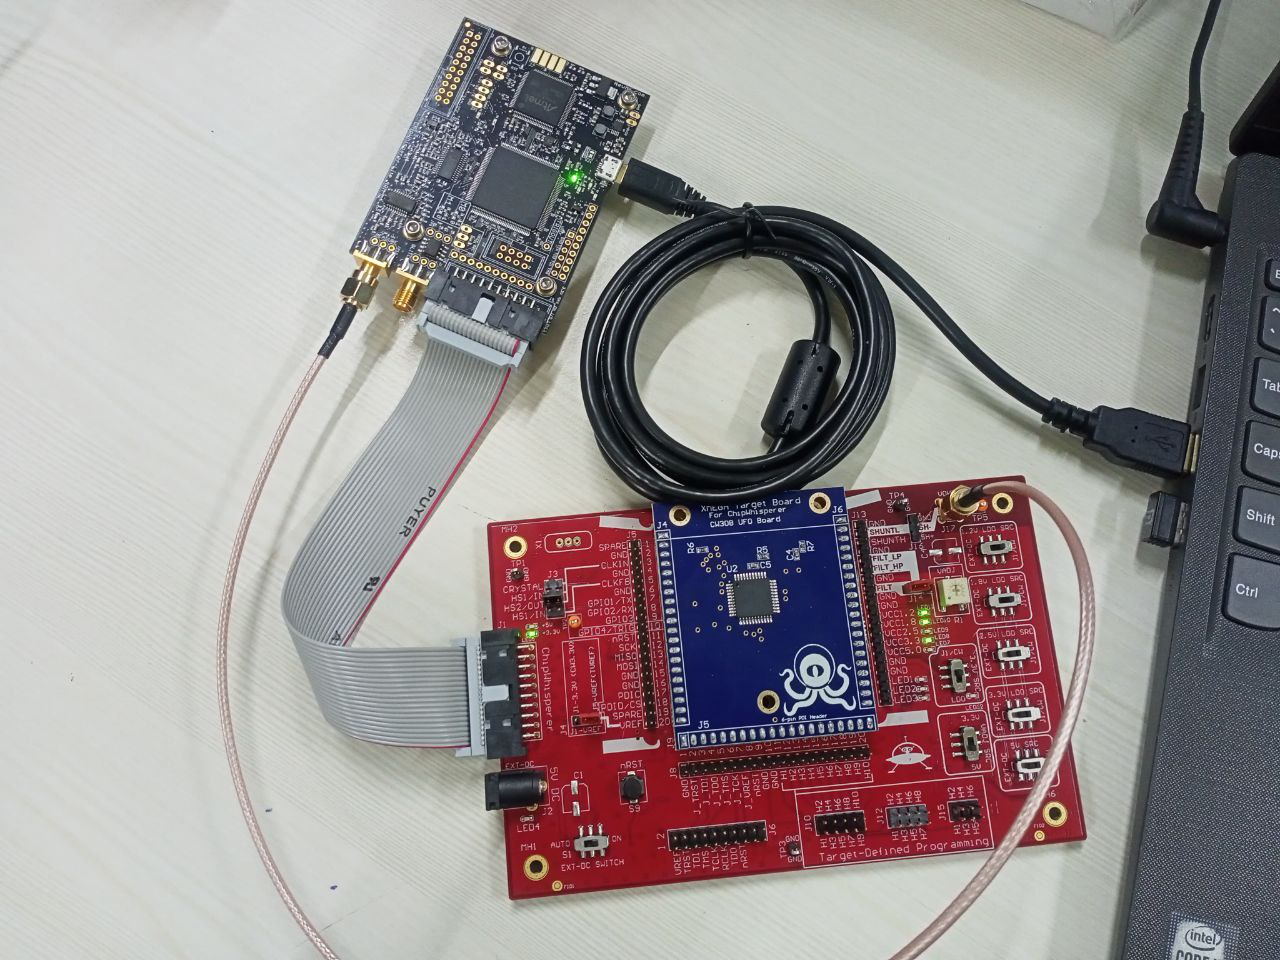
\includegraphics[width=\linewidth]{images/cwlite_separated_background.JPEG}
    \smallskip
    \textbf{CWLite with Separate Target}
  \end{minipage}
  \hfill
  \begin{minipage}[b]{0.3\linewidth}
    \centering
    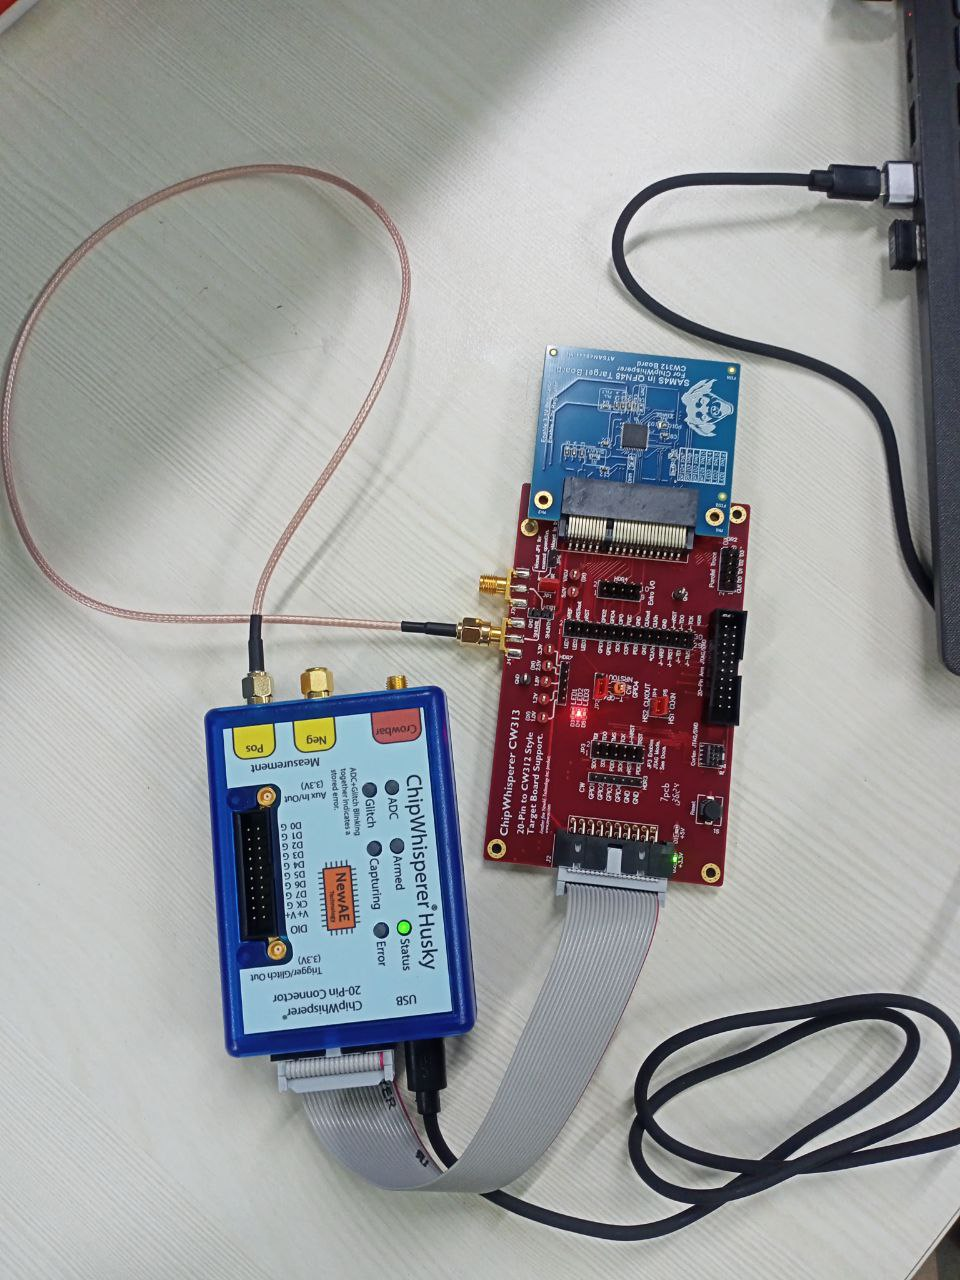
\includegraphics[width=\linewidth]{images/cwhusky_background.JPEG}
    \smallskip
    \textbf{CWHusky setup}
  \end{minipage}
\end{frame}

\begin{frame}[fragile]{CWLite with ARM 32-bit Target}
  \centering
  \begin{itemize}
    \item 10-bit 105MS/s ADC for capturing power traces
    \item Clock and voltage fault generation via FPGA-based pulse generation
    \item Sample Buffer Size:	24,573 samples
    \item Capable of doing both Voltage glitching and clock glitching
  \end{itemize}
  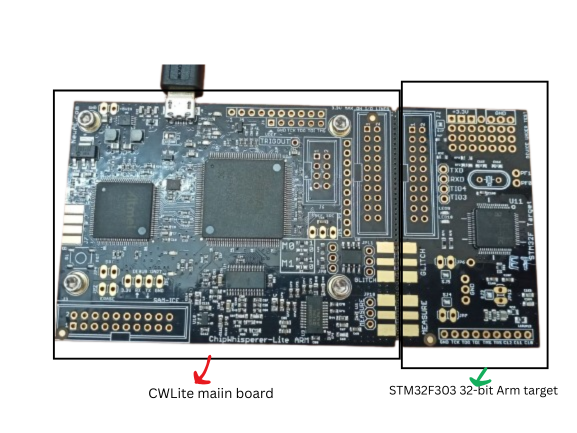
\includegraphics[width=0.6\linewidth]{images/cwlite.png}
  \smallskip

  

\end{frame}

\begin{frame}{Software Environment}
  
  
\end{frame}
\subsection{Softeware Environment}
\subsection{Steps to inject a Fault using ChipWhisperer}

\section{Real-world Replication of the State-of-the-Art}
\begin{frame}{Diagonals in the AES}
  \[
\begin{array}{cc}
\textbf{Diagonal 0}~[D_0] & \textbf{Diagonal 1}~[D_1] \\[1ex]
\begin{array}{|c|c|c|c|}
\hline
\fcolorbox{red}{red!20}{$a_{00}$} & a_{01} & a_{02} & a_{03} \\
\hline
a_{10} & \fcolorbox{red}{red!20}{$a_{11}$} & a_{12} & a_{13} \\
\hline
a_{20} & a_{21} & \fcolorbox{red}{red!20}{$a_{22}$} & a_{23} \\
\hline
a_{30} & a_{31} & a_{32} & \fcolorbox{red}{red!20}{$a_{33}$} \\
\hline
\end{array}
&
\begin{array}{|c|c|c|c|}
\hline
a_{00} & \fcolorbox{blue}{blue!20}{$a_{01}$} & a_{02} & a_{03} \\
\hline
a_{10} & a_{11} & \fcolorbox{blue}{blue!20}{$a_{12}$} & a_{13} \\
\hline
a_{20} & a_{21} & a_{22} & \fcolorbox{blue}{blue!20}{$a_{23}$} \\
\hline
\fcolorbox{blue}{blue!20}{$a_{30}$} & a_{31} & a_{32} & a_{33} \\
\hline
\end{array}
\\[6ex]
\textbf{Diagonal 2}~[D_2] & \textbf{Diagonal 3}~[D_3] \\[1ex]
\begin{array}{|c|c|c|c|}
\hline
a_{00} & a_{01} & \fcolorbox{green!50!black}{green!20}{$a_{02}$} & a_{03} \\
\hline
a_{10} & a_{11} & a_{12} & \fcolorbox{green!50!black}{green!20}{$a_{13}$} \\
\hline
\fcolorbox{green!50!black}{green!20}{$a_{20}$} & a_{21} & a_{22} & a_{23} \\
\hline
a_{30} & \fcolorbox{green!50!black}{green!20}{$a_{31}$} & a_{32} & a_{33} \\
\hline
\end{array}
&
\begin{array}{|c|c|c|c|}
\hline
a_{00} & a_{01} & a_{02} & \fcolorbox{orange!80!black}{orange!20}{$a_{03}$} \\
\hline
\fcolorbox{orange!80!black}{orange!20}{$a_{10}$} & a_{11} & a_{12} & a_{13} \\
\hline
a_{20} & \fcolorbox{orange!80!black}{orange!20}{$a_{21}$} & a_{22} & a_{23} \\
\hline
a_{30} & a_{31} & \fcolorbox{orange!80!black}{orange!20}{$a_{32}$} & a_{33} \\
\hline
\end{array}
\end{array}
\]
  
\end{frame}
\begin{frame}{Fault Injection at the Start of Round 8 using CW-Lite}
  \begin{figure}
    \centering
    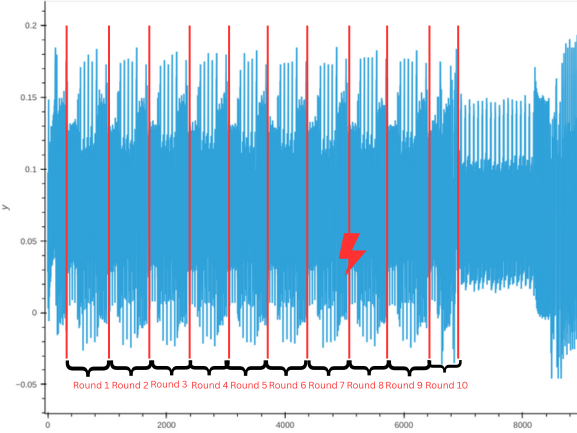
\includegraphics[width=0.7\linewidth]{images/aes128_powertrace.png}
    \caption{Power Trace of AES128}
  \end{figure}
\end{frame}
\begin{frame}[fragile]{Using Clock Glitching}
  \textbf{Target:} AES-128 on CWLite-ARM
  
  \vspace{1mm}
  \begin{itemize}
    \item 8th round identified at sample range: \textbf{5080–5120}
    \item Clock glitch injected at: \textbf{5086 samples}
  \end{itemize}
  
  \textbf{Glitch Configuration:}
  \vspace{1mm}
  
  \begin{lstlisting}
  scope.glitch.clk_src = "clkgen"
  scope.glitch.output = "clock_xor"
  scope.glitch.trigger_src = "ext_single"
  scope.glitch.repeat = 1
  scope.io.hs2 = "glitch"
  scope.glitch.offset = 10
  scope.glitch.width = 3
  \end{lstlisting}
  
  \textbf{Result:}
  \begin{itemize}
    \item Faulty Ciphertext: \texttt{56 9b 6f 66 c9 41 96 f7 9c f1 49 44 29 13 04 e4}
    \item Correct Ciphertext: \texttt{f5 d3 d5 85 03 b9 69 9d e7 85 89 5a 96 fd ba af}
  \end{itemize}
  \end{frame}

  \begin{frame}[fragile]{AES Fault Analysis: Rounds 8–10}
    \scriptsize % or \tiny for even smaller
    
    \textbf{After Fault Injection at Start of $8^{\text{th}}$ Round}
    \[
    \begin{array}{ccc}
    \textbf{No Fault} & \textbf{With Fault} & \textbf{Diff} \\
    \begin{array}{|c|c|c|c|} \hline
    96 & e9 & e9 & 3c \\ \hline
    71 & 87 & 61 & 89 \\ \hline
    6a & 91 & 04 & 13 \\ \hline
    e4 & c7 & 90 & ff \\ \hline
    \end{array}
    &
    \begin{array}{|c|c|c|c|} \hline
    96 & e9 & e9 & 3c \\ \hline
    71 & a3 & 61 & 89 \\ \hline
    6a & 91 & 04 & 13 \\ \hline
    e4 & c7 & 90 & ff \\ \hline
    \end{array}
    &
    \begin{array}{|c|c|c|c|} \hline
    00 & 00 & 00 & 00 \\ \hline
    00 & \fcolorbox{red}{red!20}{24} & 00 & 00 \\ \hline
    00 & 00 & 00 & 00 \\ \hline
    00 & 00 & 00 & 00 \\ \hline
    \end{array}
    \end{array}
    \]
    
    \vspace{1mm}
    \textbf{After Round 8 (SubBytes, ShiftRows, MixColumns, AddRoundKey)}
    \[
    \begin{array}{ccc}
    \begin{array}{|c|c|c|c|} \hline
    0c & b7 & 3b & ad \\ \hline
    77 & b8 & a0 & c3 \\ \hline
    31 & 0a & 19 & d8 \\ \hline
    43 & b0 & 70 & eb \\ \hline
    \end{array}
    &
    \begin{array}{|c|c|c|c|} \hline
    2b & b7 & 3b & ad \\ \hline
    4d & b8 & a0 & c3 \\ \hline
    2c & 0a & 19 & d8 \\ \hline
    5e & b0 & 70 & eb \\ \hline
    \end{array}
    &
    \begin{array}{|c|c|c|c|} \hline
    \fcolorbox{red}{red!20}{27} & 00 & 00 & 00 \\ \hline
    \fcolorbox{red}{red!20}{3a} & 00 & 00 & 00 \\ \hline
    \fcolorbox{red}{red!20}{1d} & 00 & 00 & 00 \\ \hline
    \fcolorbox{red}{red!20}{1d} & 00 & 00 & 00 \\ \hline
    \end{array}
    \end{array}
    \]
    \end{frame}
    \begin{frame}[fragile]{AES Fault Analysis: Rounds 8–10}
    \scriptsize
    \textbf{After Round 9}
    \[
    \begin{array}{ccc}
    \begin{array}{|c|c|c|c|} \hline
    c2 & 10 & a5 & 54 \\ \hline
    df & 31 & da & c0 \\ \hline
    67 & 79 & 42 & 5d \\ \hline
    9b & 74 & 40 & fa \\ \hline
    \end{array}
    &
    \begin{array}{|c|c|c|c|} \hline
    dc & 52 & 13 & 6e \\ \hline
    d0 & 73 & 1b & ec \\ \hline
    68 & bf & 35 & 4b \\ \hline
    8a & f0 & f6 & ec \\ \hline
    \end{array}
    &
    \begin{array}{|c|c|c|c|} \hline
    \fcolorbox{red}{red!20}{1e} & \fcolorbox{red}{red!20}{42} & \fcolorbox{red}{red!20}{b6} & \fcolorbox{red}{red!20}{3a} \\ \hline
    \fcolorbox{red}{red!20}{0f} & \fcolorbox{red}{red!20}{42} & \fcolorbox{red}{red!20}{c1} & \fcolorbox{red}{red!20}{2c} \\ \hline
    \fcolorbox{red}{red!20}{0f} & \fcolorbox{red}{red!20}{c6} & \fcolorbox{red}{red!20}{77} & \fcolorbox{red}{red!20}{16} \\ \hline
    \fcolorbox{red}{red!20}{11} & \fcolorbox{red}{red!20}{84} & \fcolorbox{red}{red!20}{b6} & \fcolorbox{red}{red!20}{16} \\ \hline
    \end{array}
    \end{array}
    \]
    
    \vspace{1mm}
    \textbf{After Round 10 (Final Output)}
    \[
    \begin{array}{ccc}
    \textbf{Correct Ciphertext} & \textbf{Faulty Ciphertext} & \textbf{Difference} \\
    \begin{array}{|c|c|c|c|} \hline
    f5 & 03 & e7 & 96 \\ \hline
    d3 & b9 & 85 & fd \\ \hline
    d5 & 69 & 89 & ba \\ \hline
    85 & 9d & 5a & af \\ \hline
    \end{array}
    &
    \begin{array}{|c|c|c|c|} \hline
    56 & c9 & 9c & 29 \\ \hline
    9b & 41 & f1 & 13 \\ \hline
    6f & 96 & 49 & 04 \\ \hline
    66 & f7 & 44 & e4 \\ \hline
    \end{array}
    &
    \begin{array}{|c|c|c|c|} \hline
    \fcolorbox{red}{red!20}{a3} & \fcolorbox{red}{red!20}{ca} & \fcolorbox{red}{red!20}{7b} & \fcolorbox{red}{red!20}{bf} \\ \hline
    \fcolorbox{red}{red!20}{48} & \fcolorbox{red}{red!20}{f8} & \fcolorbox{red}{red!20}{74} & \fcolorbox{red}{red!20}{ee} \\ \hline
    \fcolorbox{red}{red!20}{ba} & \fcolorbox{red}{red!20}{ff} & \fcolorbox{red}{red!20}{c0} & \fcolorbox{red}{red!20}{be} \\ \hline
    \fcolorbox{red}{red!20}{e3} & \fcolorbox{red}{red!20}{6a} & \fcolorbox{red}{red!20}{1e} & \fcolorbox{red}{red!20}{4b} \\ \hline
    \end{array}
    \end{array}
    \]
    
    \end{frame}
\begin{frame}
    \scriptsize
    \[
\begin{array}{ccc}
    \textbf{After 8th Round} & \textbf{After 9th Round} & \textbf{After 10th Round Shift Row} \\[1ex]
    \begin{array}{|c|c|c|c|}
        \hline
        \texttt{$f_1$} & \texttt{ } & \texttt{ } &  \texttt{ }\\
        \hline
        \texttt{$f_2$} & \texttt{ } & \texttt{ } &  \texttt{ }  \\
        \hline
        \texttt{$f_3$} & \texttt{ } & \texttt{ } &  \texttt{ }  \\
        \hline
        \texttt{$f_4$}& \texttt{ } & \texttt{ } &  \texttt{ }  \\
        \hline
    \end{array}
&

\begin{array}{|c|c|c|c|}
    \hline
    \texttt{2$f_1$} & \texttt{$f_4$} & \texttt{$f_3$} & \texttt{3$f_2$} \\
    \hline
    \texttt{$f_1$} & \texttt{$f_4$} & \texttt{3$f_3$} & \texttt{2$f_2$} \\
    \hline
    \texttt{$f_1$} & \texttt{3$f_4$} & \texttt{2$f_3$} & \texttt{$f_2$} \\
    \hline
    \texttt{3$f_1$} & \texttt{2$f_4$} & \texttt{$f_3$} & \texttt{$f_2$} \\
    \hline
\end{array}

    &

    \begin{array}{|c|c|c|c|}
        \hline
        \texttt{2$f_1$} & \texttt{$f_4$} & \texttt{$f_3$} & \texttt{3$f_2$} \\
        \hline
        \texttt{$f_4$} & \texttt{3$f_3$} & \texttt{2$f_2$} & \texttt{$f_1$}\\
        \hline
        \texttt{2$f_3$} & \texttt{$f_2$} & \texttt{$f_1$} & \texttt{3$f_4$} \\
        \hline
        \texttt{$f_2$} & \texttt{3$f_1$} & \texttt{2$f_4$} & \texttt{$f_3$} \\
        \hline
    \end{array}
    
\end{array}
\]
If we represent the $10^{th}$ round key as \(K_{10}\), it can be expressed as:
\[
    \begin{array}{|c|c|c|c|}
        \hline
        k_{00} & k_{01} & k_{02} & k_{03} \\
        \hline
        k_{10} & k_{11} & k_{12} & k_{13} \\
        \hline
        k_{20} & k_{21} & k_{22} & k_{23} \\
        \hline
        k_{30} & k_{31} & k_{32} & k_{33} \\
        \hline
        \end{array}
\]
  \end{frame}
\begin{frame}[fragile]{Using Voltage Glitching}
    \textbf{Target:} AES-128 on CWLite-ARM
    
    \vspace{1mm}
    \begin{itemize}
      \item 8th round identified at sample range: \textbf{5080–5120}
      \item Clock glitch injected at: \textbf{5100 samples}
    \end{itemize}
    
    \textbf{Glitch Configuration:}
    \vspace{1mm}
    
    \begin{lstlisting}
      scope.glitch.clk_src = "clkgen"
      scope.glitch.output = "glitch_only"
      scope.glitch.trigger_src = "ext_single"
      scope.io.glitch_lp = True
      scope.io.glitch_hp = True
      scope.glitch.offset = -37.890625
      scope.glitch.width  = 37.109375
    \end{lstlisting}
    
    \textbf{Result:}
    \begin{itemize}
      \item Faulty Ciphertext: \texttt{5d 37 58 b2 4b b2 0b 7c 9e 67 58 55 39 b0 2d ab}
      \item Correct Ciphertext: \texttt{f5 d3 d5 85 03 b9 69 9d e7 85 89 5a 96 fd ba af}
    \end{itemize}
    \end{frame}
  
\begin{frame}[fragile]{AES Fault Analysis: Rounds 8–10}
      \scriptsize % or \tiny for even smaller
      
    \vspace{1ex}
    \textbf{After Fault Injection at Start of 8\textsuperscript{th} Round}
    \[
    \setlength{\arraycolsep}{2pt}
    \renewcommand{\arraystretch}{1.1}
    \begin{array}{ccc}
    \textbf{Without Fault} & \textbf{With Fault} & \textbf{Difference} \\
    
    \begin{array}{|c|c|c|c|}
    \hline \texttt{96} & \texttt{e9} & \texttt{e9} & \texttt{3c} \\
    \hline \texttt{71} & \texttt{87} & \texttt{61} & \texttt{89} \\
    \hline \texttt{6a} & \texttt{91} & \texttt{04} & \texttt{13} \\
    \hline \texttt{e4} & \texttt{c7} & \texttt{90} & \texttt{ff} \\
    \hline
    \end{array}
    &
    
    \begin{array}{|c|c|c|c|}
    \hline \texttt{96} & \texttt{e9} & \texttt{e9} & \texttt{52} \\
    \hline \texttt{52} & \texttt{87} & \texttt{61} & \texttt{89} \\
    \hline \texttt{6a} & \texttt{91} & \texttt{04} & \texttt{13} \\
    \hline \texttt{e4} & \texttt{c7} & \texttt{90} & \texttt{ff} \\
    \hline
    \end{array}
    &
    
    \begin{array}{|c|c|c|c|}
    \hline \texttt{00} & \texttt{00} & \texttt{00} & \fcolorbox{orange!80!black}{orange!20}{\texttt{6e}} \\
    \hline \fcolorbox{orange!80!black}{orange!20}{\texttt{23}} & \texttt{00} & \texttt{00} & \texttt{00} \\
    \hline \texttt{00} & \texttt{00} & \texttt{00} & \texttt{00} \\
    \hline \texttt{00} & \texttt{00} & \texttt{00} & \texttt{00} \\
    \hline
    \end{array}
    \end{array}
    \]
    
    \vspace{0.5em}
    \textbf{After Completion of 8\textsuperscript{th} RoundSubByte,ShiftRow,MixColumn,AddRoundkey(8)}
    \[
    \begin{array}{ccc}
    \textbf{Without Fault} & \textbf{With Fault} & \textbf{Difference} \\
    
    \begin{array}{|c|c|c|c|}
    \hline \texttt{0c} & \texttt{b7} & \texttt{3b} & \texttt{ad} \\
    \hline \texttt{77} & \texttt{b8} & \texttt{a0} & \texttt{c3} \\
    \hline \texttt{31} & \texttt{0a} & \texttt{19} & \texttt{d8} \\
    \hline \texttt{43} & \texttt{b0} & \texttt{70} & \texttt{eb} \\
    \hline
    \end{array}
    &
    \begin{array}{|c|c|c|c|}
    \hline \texttt{0c} & \texttt{b7} & \texttt{3b} & \texttt{9e} \\
    \hline \texttt{77} & \texttt{b8} & \texttt{a0} & \texttt{75} \\
    \hline \texttt{31} & \texttt{0a} & \texttt{19} & \texttt{90} \\
    \hline \texttt{43} & \texttt{b0} & \texttt{70} & \texttt{6e} \\
    \hline
    \end{array}
    &
    \begin{array}{|c|c|c|c|}
    \hline \texttt{00} & \texttt{00} & \texttt{00} & \fcolorbox{orange!80!black}{orange!20}{\texttt{33}} \\
    \hline \texttt{00} & \texttt{00} & \texttt{00} & \fcolorbox{orange!80!black}{orange!20}{\texttt{b6}} \\
    \hline \texttt{00} & \texttt{00} & \texttt{00} & \fcolorbox{orange!80!black}{orange!20}{\texttt{48}} \\
    \hline \texttt{00} & \texttt{00} & \texttt{00} & \fcolorbox{orange!80!black}{orange!20}{\texttt{85}} \\
    \hline
    \end{array}
    \end{array}
    \]
    \end{frame}
\begin{frame}[fragile]{AES Fault Analysis: Rounds 8–10}
    \scriptsize
    \textbf{After The Completion of $9^{\text{th}}$ Round(SubByte,ShiftRow,MixColumn,AddRoundkey(9))}
\[
\begin{array}{ccc}
\textbf{Without Fault} & \textbf{With Fault } & \textbf{Difference } \\[1ex]
\begin{array}{|c|c|c|c|}
    \hline
    \texttt{c2} & \texttt{10} & \texttt{a5} & \texttt{54} \\
    \hline
    \texttt{df} & \texttt{31} & \texttt{da} & \texttt{c0} \\
    \hline
    \texttt{67} & \texttt{79} & \texttt{42} & \texttt{5d} \\
    \hline
    \texttt{9b} & \texttt{74} & \texttt{40} & \texttt{fa} \\
    \hline
\end{array} 
&

\begin{array}{|c|c|c|c|}
    \hline
    \texttt{b4} & \texttt{11} & \texttt{6b} & \texttt{73} \\
    \hline
    \texttt{a9} & \texttt{32} & \texttt{a7} & \texttt{5e} \\
    \hline
    \texttt{fd} & \texttt{7b} & \texttt{f1} & \texttt{c3} \\
    \hline
    \texttt{77} & \texttt{75} & \texttt{f3} & \texttt{43} \\
    \hline
    \end{array}

    &

    \begin{array}{|c|c|c|c|}
        \hline
        \fcolorbox{orange!80!black}{orange!20}{\texttt{76}} & \fcolorbox{orange!80!black}{orange!20}{\texttt{01}} & \fcolorbox{orange!80!black}{orange!20}{\texttt{ce}} & \fcolorbox{orange!80!black}{orange!20}{\texttt{27}} \\
        \hline
        \fcolorbox{orange!80!black}{orange!20}{\texttt{76}} & \fcolorbox{orange!80!black}{orange!20}{\texttt{03}} & \fcolorbox{orange!80!black}{orange!20}{\texttt{7d}} & \fcolorbox{orange!80!black}{orange!20}{\texttt{9e}} \\
        \hline
        \fcolorbox{orange!80!black}{orange!20}{\texttt{9a}} & \fcolorbox{orange!80!black}{orange!20}{\texttt{02}} & \fcolorbox{orange!80!black}{orange!20}{\texttt{b3}} & \fcolorbox{orange!80!black}{orange!20}{\texttt{9e}} \\
        \hline
        \fcolorbox{orange!80!black}{orange!20}{\texttt{ec}} & \fcolorbox{orange!80!black}{orange!20}{\texttt{01}} & \fcolorbox{orange!80!black}{orange!20}{\texttt{b3}} & \fcolorbox{orange!80!black}{orange!20}{\texttt{b9}} \\
        \hline
    \end{array}
\end{array}
\]
\textbf{After The Completion of $10^{\text{th}}$ Round(SubByte,ShiftRow,AddRoundkey(10)) :}
\[
\begin{array}{ccc}
\textbf{Without Fault} & \textbf{With Fault } & \textbf{Difference } \\[1ex]
\begin{array}{|c|c|c|c|}
    \hline
    \texttt{f5} & \texttt{03} & \texttt{e7} & \texttt{96} \\
    \hline
    \texttt{d3} & \texttt{b9} & \texttt{85} & \texttt{fd} \\
    \hline
    \texttt{d5} & \texttt{69} & \texttt{89} & \texttt{ba} \\
    \hline
    \texttt{85} & \texttt{9d} & \texttt{5a} & \texttt{af} \\
    \hline
\end{array} 
&

\begin{array}{|c|c|c|c|}
    \hline
    \texttt{5d} & \texttt{4b} & \texttt{9e} & \texttt{39} \\
    \hline
    \texttt{37} & \texttt{b2} & \texttt{67} & \texttt{b0} \\
    \hline
    \texttt{58} & \texttt{0b} & \texttt{58} & \texttt{2d} \\
    \hline
    \texttt{b2} & \texttt{7c} & \texttt{55} & \texttt{ab} \\
    \hline
    \end{array}

    &

\begin{array}{|c|c|c|c|}
    \hline
    \fcolorbox{orange!80!black}{orange!20}{\texttt{a8}} & \fcolorbox{orange!80!black}{orange!20}{\texttt{48}} & \fcolorbox{orange!80!black}{orange!20}{\texttt{79}} & \fcolorbox{orange!80!black}{orange!20}{\texttt{af}} \\
    \hline
    \fcolorbox{orange!80!black}{orange!20}{\texttt{e4}} & \fcolorbox{orange!80!black}{orange!20}{\texttt{0b}} & \fcolorbox{orange!80!black}{orange!20}{\texttt{e2}} & \fcolorbox{orange!80!black}{orange!20}{\texttt{4d}} \\
    \hline
    \fcolorbox{orange!80!black}{orange!20}{\texttt{8d}} & \fcolorbox{orange!80!black}{orange!20}{\texttt{62}} & \fcolorbox{orange!80!black}{orange!20}{\texttt{d1}} & \fcolorbox{orange!80!black}{orange!20}{\texttt{97}} \\
    \hline
    \fcolorbox{orange!80!black}{orange!20}{\texttt{37}} & \fcolorbox{orange!80!black}{orange!20}{\texttt{e1}} & \fcolorbox{orange!80!black}{orange!20}{\texttt{0f}} & \fcolorbox{orange!80!black}{orange!20}{\texttt{04}} \\
    \hline
    \end{array}
\end{array}
\]
\end{frame}

\begin{frame}[fragile]
\scriptsize
\[
\begin{array}{ccc}
    \textbf{After 8th Round} & \textbf{After 9th Round} & \textbf{After 10th Round Shift Row} \\[1ex]
    \begin{array}{|c|c|c|c|}
        \hline
        \texttt{ } & \texttt{ } & \texttt{ } & \texttt{$f_1$} \\
        \hline
        \texttt{ } & \texttt{ } & \texttt{ } & \texttt{$f_2$} \\
        \hline
        \texttt{ } & \texttt{ } & \texttt{ } & \texttt{$f_3$} \\
        \hline
        \texttt{ } & \texttt{ } & \texttt{ } & \texttt{$f_4$} \\
        \hline
    \end{array}
    &

    \begin{array}{|c|c|c|c|}
        \hline
        \texttt{$f_4$} & \texttt{$f_3$} & \texttt{3$f_2$} & \texttt{2$f_1$} \\
        \hline
        \texttt{$f_4$} & \texttt{3$f_3$} & \texttt{2$f_2$} & \texttt{$f_1$} \\
        \hline
        \texttt{3$f_4$} & \texttt{2$f_3$} & \texttt{$f_2$} & \texttt{$f_1$} \\
        \hline
        \texttt{2$f_4$} & \texttt{$f_3$} & \texttt{$f_2$} & \texttt{3$f_1$} \\
        \hline
    \end{array}
    &

    \begin{array}{|c|c|c|c|}
        \hline
        \texttt{$f_4$} & \texttt{$f_3$} & \texttt{3$f_2$} & \texttt{2$f_1$} \\
        \hline
        \texttt{3$f_3$} & \texttt{2$f_2$} & \texttt{$f_1$} & \texttt{$f_4$} \\
        \hline
        \texttt{$f_2$} & \texttt{$f_1$} & \texttt{3$f_4$} & \texttt{2$f_3$} \\
        \hline
        \texttt{3$f_1$} & \texttt{2$f_4$} & \texttt{$f_3$} & \texttt{$f_2$} \\
        \hline
    \end{array}
\end{array}
\]
If we represent the $10^{th}$ round key as \(K_{10}\), it can be expressed as:
\[
    \begin{array}{|c|c|c|c|}
        \hline
        k_{00} & k_{01} & k_{02} & k_{03} \\
        \hline
        k_{10} & k_{11} & k_{12} & k_{13} \\
        \hline
        k_{20} & k_{21} & k_{22} & k_{23} \\
        \hline
        k_{30} & k_{31} & k_{32} & k_{33} \\
        \hline
        \end{array}
\]
\end{frame}


\section{Flipping Bits to Break BipBip}
\begin{frame}[fragile]
    \textbf{Key Points about BipBip Cipher}
    \begin{itemize}
        \item \textbf{Tweakable block cipher} tailored for fast decryption in ASICs.
        \item Uses an unconventional \textbf{24-bit block size}, a \textbf{256-bit master key}, and a \textbf{40-bit tweak}.
        \item Optimized for latency-sensitive applications (e.g., embedded systems, IoT).
        \item \textbf{Decryption-oriented design} — emphasizes ciphertext-to-plaintext transformation.
        \item \textbf{Decryption Structure Overview:}
        \begin{figure}[h]
          \centering
          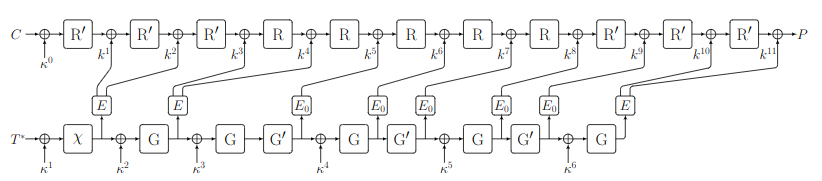
\includegraphics[width=0.9\textwidth]{images/bipbip.png}
          \caption{High Level Decryption Structure of BipBip}
          \label{fig:bipbip_decrypt_structure}
        \end{figure}
        \end{itemize}
\end{frame}

\begin{frame}[fragile]{Attack Model}
  \begin{figure}[h]
    \centering
    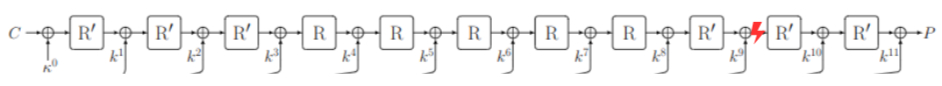
\includegraphics[width=0.9\textwidth]{images/bipbip_attack.png}
    \caption{Proposed fault injection attack}
    \label{fig:bipbip_attack}
\end{figure}
\begin{itemize}
\item A single bit fault at the start of 9th round s-box operation is required. 
\item Need such 4 Faulty values where single bit is flipped in the input of 9th round s-box.
\end{itemize}
\end{frame}
\begin{frame}[fragile]{Power Trace of BipBip on CWLite-ARM}
  \begin{figure}[h]
    \centering
    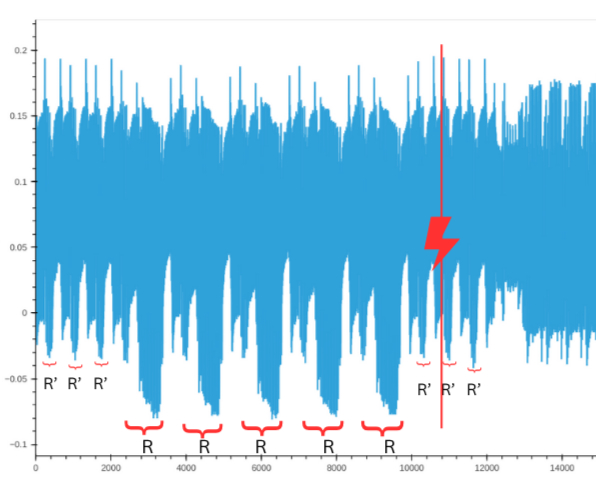
\includegraphics[width=0.7\textwidth]{images/bipbip_powertrace.png}
    \caption{Power trace BipBip on CWLite-ARM}
    \label{fig:bipbip_powertrace}
\end{figure}
\end{frame}

\begin{frame}[fragile]{Glitch Attack Settings on BipBip Implementation}
\begin{itemize}
    \item \textbf{Initial Step:} Integrated \texttt{sempleserial} for communication between target and scope.
    \item \textbf{Attack Window:} Identified using BipBip power trace on CWLite — approx.\ between samples \texttt{10820 to 10890}.
    \item \textbf{CWLite Settings:}
    \begin{itemize}
        \item \texttt{scope.glitch.clk_src = "clkgen"}
        \item \texttt{scope.glitch.output = "clock_xor"}
        \item \texttt{scope.glitch.trigger_src = "ext_single"}
        \item \texttt{scope.glitch.repeat = 1}
        \item \texttt{scope.io.hs2 = "glitch"}
    \end{itemize}
    \item \textbf{CWHusky Settings:}
    \begin{itemize}
        \item \texttt{scope.glitch.clk_src = "pll"}
    \end{itemize}
    \item Attack location on CWHusky determined from BipBip's power trace on that platform.
\end{itemize}
\end{frame}

\begin{frame}{Analysis of the attack}
  \tiny
  \begin{table}[h!]
    \centering
    \tiny % Reduce font size to make it fit better
    \caption{Summary of Clock Glitch Fault Injection Parameters and Results}
    \begin{tabular}{|c|c|c|c|p{5.5cm}|} % narrower last column
    \hline
    \textbf{Location} & \textbf{Width} & \textbf{Offset} & \textbf{Plaintext} & \textbf{Faulty vs Correct state (Input of Round 9)} \\
    \hline
    10841 & 1.17 & 1.17 & 052aa7 & 
    \parbox{5.5cm}{
        \text{}\\
        \textbf{Faulty:} 0\textcolor{red}{1}1100 100111 111101 101111\\
        \textbf{Correct:} 0\textcolor{green}{0}1100\ \ 100111\ 111101\ 101111 \\
    } \\
    \hline
    10842 & 1.95 & 1.17 & 6462d1 & 
    \parbox{5.5cm}{
        \text{}\\
        \textbf{Faulty:} 00\textcolor{red}{0}100 100111 111101 101111\\
        \textbf{Correct:} 00\textcolor{green}{1}100\ \ 100111\ 111101\ 101111 \\
    } \\
    \hline
    10855 & 1.9 & 1.7 & 6f2a99 &
    \parbox{5.5cm}{
        \text{}\\
        \textbf{Faulty:} 001\textcolor{red}{0}00\ 100111\ 111101\ 101111 \\
       \textbf{Correct:} 001\textcolor{green}{1}00\ 100111\ 111101\ 101111 \\

    } \\
    \hline
    10866 & 1.17 & 1.17 & 3c12bc & 
    \parbox{5.5cm}{
        \text{}\\
        \textbf{Faulty:} 00110\textcolor{red}{1}\ 100111\ 111101\ 101111 \\
        \textbf{Correct:} 00110\textcolor{green}{0}\ 100111\ 111101\ 101111 \\

    } \\
    \hline
    10878 & 1.17 & 1.17 & 105bfc & 
    \parbox{5.5cm}{
        \text{}\\
        \textbf{Faulty:} 001100\ 1001\textcolor{red}{0}1\ 111101\ 101111 \\
        \textbf{Correct:} 001100\ 1001\textcolor{green}{1}1\ 111101\ 101111 \\

    } \\
    \hline
    10887 & 1.9 & 1.17 & 1c52e4 & 
    \parbox{5.5cm}{
        \text{}\\
        \textbf{Faulty:} 001100\ 10\textcolor{red}{1}111\ 111101\ 101111 \\
        \textbf{Correct:} 001100\ 10\textcolor{green}{0}111\ 111101\ 101111 \\

    } \\
    \hline
    \end{tabular}
    \label{tab:glitch_summary}
    \end{table}

\end{frame}
\section{Preparing PQC for Fault Analysis: A Kyber Implementation}
\begin{frame}{NIST PQC Standardization Overview}
  \small
  \begin{itemize}
    \item \textbf{Goal:} Identify quantum-resistant public-key cryptographic algorithms for standardization.
    
    \item \textbf{Initiated:} December 2016 by NIST in response to the threat posed by quantum computers.

    \item \textbf{Process:}
    \begin{itemize}
      \item Round 1: 69 submissions (Dec 2017)
      \item Round 2: 26 candidates (Jan 2019)
      \item Round 3: 7 finalists + 8 alternates (July 2020)
      \item \textbf{Final Selections (July 2022):}
      \begin{itemize}
        \item \textbf{Encryption/KEM:} \textcolor{blue}{Kyber (CRYSTALS-Kyber)}
        \item \textbf{Signatures:} \textcolor{blue}{Dilithium, Falcon, SPHINCS+}
      \end{itemize}
    \end{itemize}

    \item \textbf{Importance:} Ensures secure communication in a post-quantum world, replacing RSA and ECC.
  \end{itemize}
\end{frame}

\begin{frame}{Detailed Comparison of Kyber Variants}
  \centering
  \resizebox{\textwidth}{!}{%
    \begin{tabular}{lcccc}
      \toprule
      \textbf{Variant} & \textbf{Security Level (bits)} & \textbf{Public Key (bytes)} & \textbf{Private Key (bytes)} & \textbf{Ciphertext (bytes)} \\
      \midrule
      Kyber512 & 128 & 800 & 1,632 & 768 \\
      Kyber768 & 192 & 1,184 & 2,400 & 1,088 \\
      Kyber1024 & 256 & 1,568 & 3,168 & 1,568 \\
      \bottomrule
    \end{tabular}
  }
\end{frame}

\section{Future Work}

\end{document}
